\documentclass{article}
\usepackage[utf8]{inputenc}
\usepackage[a4paper, total={6in, 8in}]{geometry}
\title{Cosmological Evidences of Dark Matter through the CMB}
\author{Lorenzo Speri}
\date{}
%\usepackage{hyperref}
\usepackage{natbib}
\usepackage{graphicx}
% ---- Maths -------
\usepackage{amsmath}
\usepackage{amsthm}
\usepackage{physics}
% ---- Links -------
%\usepackage{hyperref}
% citation color
\usepackage[colorlinks=true,citecolor=blue]{hyperref}
% for twnsore
\usepackage{tensind}
\tensordelimiter{:}

% for comments
\usepackage{verbatim}


%  ---- my commands -------
\newcommand{\bea}{\setlength{\jot}{10pt}\begin{eqnarray*}}
\newcommand{\eea}{\end{eqnarray*}}
\newcommand{\beq}{\begin{equation}}
\newcommand{\eeq}{\end{equation}}
\newcommand{\bpsi}{\bar{\psi}}
\newcommand{\dslash}{\slashed{\partial}}
\newcommand{\Dslash}{\slashed{D}}
\newcommand{\Lagr}{\mathcal{L}}
\newcommand{\cpp}{\texttt{C++} } 
\newcommand{\mpi}{\texttt{MPI} } 
\newcommand{\de}{\nu}
\newcommand{\T}{\text{TT}}
\newcommand{\h}{\mathscr{H}}
\newcommand{\ten}{\mathscr{T}}

\begin{document}

\maketitle


\section{Introduction}
Many astronomical and cosmological observations suggest that, by using the General Theory of Relativity, there is an invisible form of matter that exerts a gravitational pull on baryonic matter. 
In order to explain such observations, scientists have proposed the existence of Dark Matter, a new form of matter that does not interact electromagnetically and, therefore, it appears invisible to us. 
The fundamental nature of Dark Matter is not well understood yet, and whether Dark Matter is truly a new form of matter or the consequence of new laws of gravity is still matter of debate.\\
One of the most compelling evidence for the existence of Dark Matter is given by the analysis of the Cosmic Microwave Background (CMB).\\
The Cosmic Microwave Background is the electromagnetic radiation coming from the hot plasma of the early stages of the Universe.
As the Universe was expanding, it cooled down to a temperature low enough to form stable hydrogen $e^- + p^+  \rightarrow H + \gamma$ (Recombination). 
As the number density of the free electrons dropped with the expansion, the Thomson scattering $e^- + \gamma  \rightarrow e^- + \gamma$ became inefficient and the photons have since streamed freely through the universe in all directions and they are today observed as the Cosmic Microwave Background \citep{LecturesPdf}.\\
The Cosmic Microwave Background appears to us as the best measured Planck spectrum that we know with fluctuations of order $10 ^{-5}$ around the average temperature $T_{CMB} =2.725$ K.
The fluctuations are extremely important because they contain the crucial information about the primordial plasma and its content. 
In fact, during the early stages of the Universe, the photons were interacting with baryonic matter, which in turn was interacting gravitationally with dark matter.
Thus, the observations of the CMB fluctuations are linked to the energy-matter content of our Universe and dark matter.\\
The aim of this paper is to give a short and concise overview of the physics of the CMB and the cosmological evidence of Dark Matter through the analysis of the CMB fluctuations within the $\Lambda$CDM model assumptions.
We are interested in providing few but fundamental tools to understand the importance of the CMB for Dark Matter.\\
We first give an historical overview of the discovery and measurements of the CMB, then we discuss the main assumptions of the $\Lambda$CDM model and the link between the content of our universe and the cosmological model. 
Afterwards, the phenomenology of the hot plasma is explained with a simplified treatment in order to understand the power spectrum of the CMB.
We conclude with the discussion of the CMB temperature power spectrum and the role of dark matter.


%The recent measurements of the Cosmic Microwave Background (CMB) radiation allowed us to infer the presence of Dark Matter in the Universe. In this summary we will explain qualitatively how the presence of Dark Matter influences the CMB anisotropies.

\section{From the Discovery of the CMB to the Planck mission}

\begin{figure}
\begin{center}
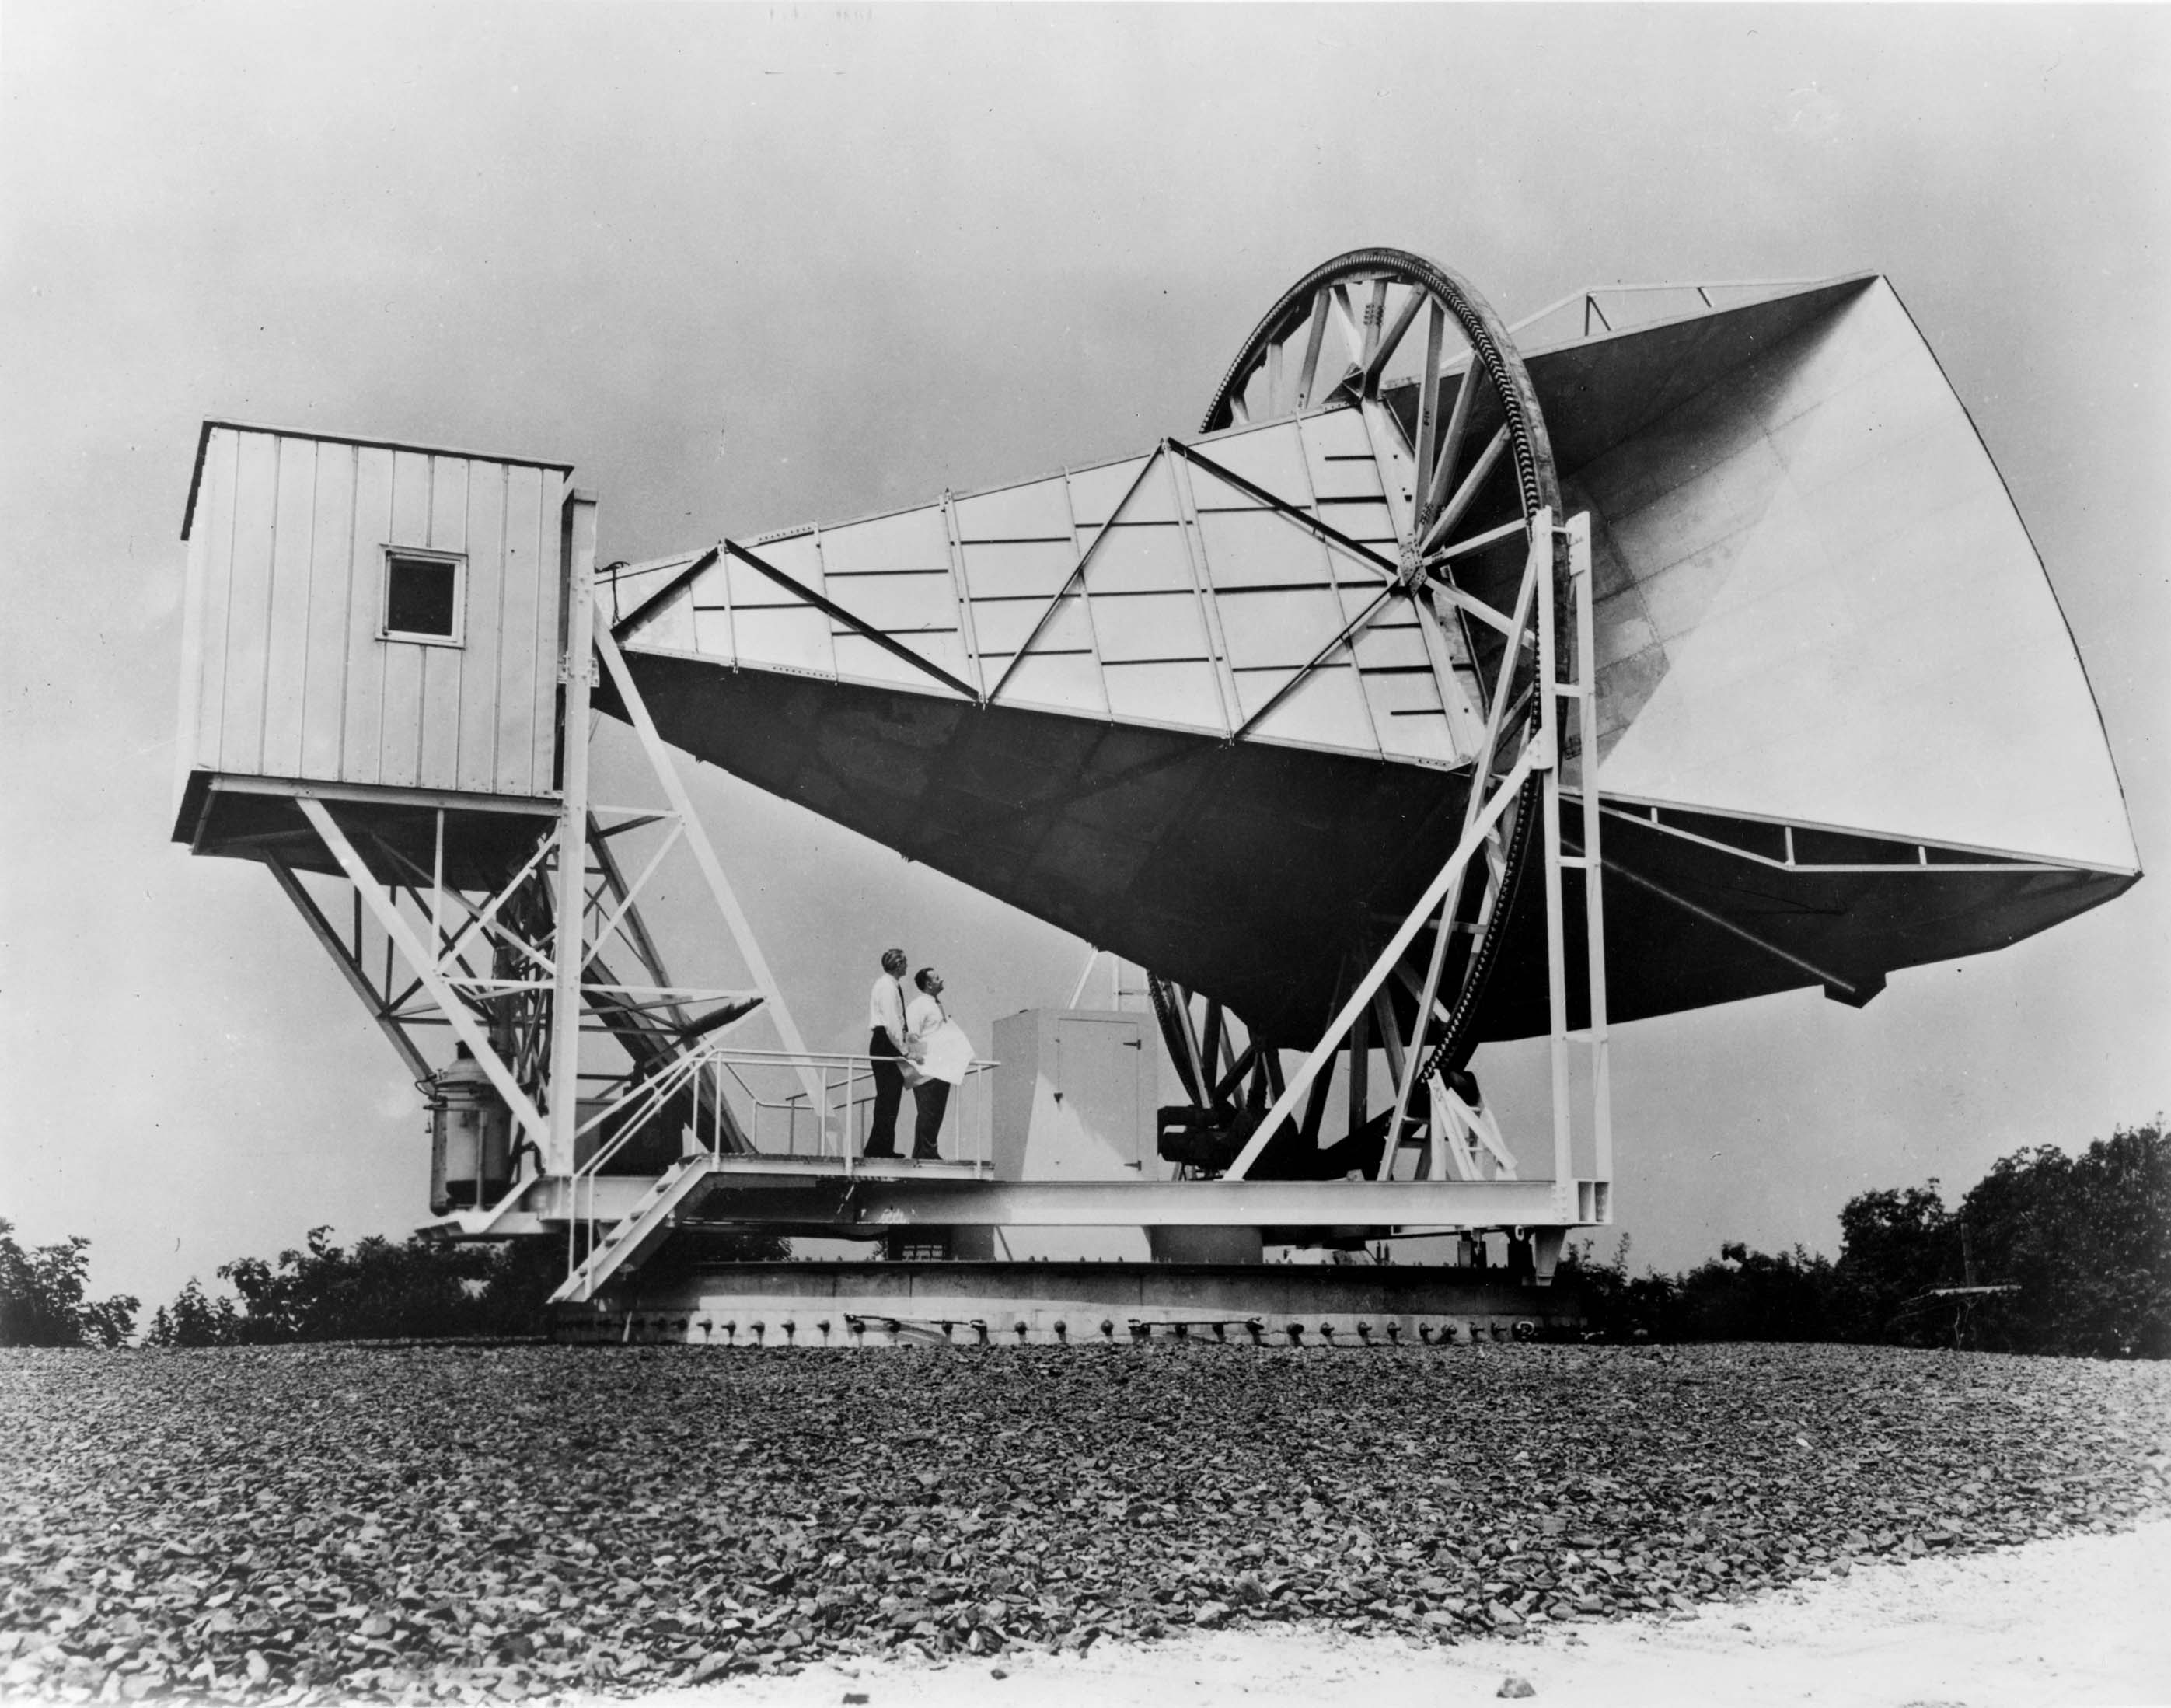
\includegraphics[width=0.7\textwidth]{Horn_Antenna.jpeg}
\caption{The 15 meter Holmdel horn antenna at Bell Telephone Laboratories in Holmdel, New Jersey.
(By NASA - Great Images in NASA Description, Public Domain, \url{https://commons.wikimedia.org/w/index.php?curid=6463768})}
\end{center}

\end{figure}

In 1965 Arno Penzias and Robert Wilson published the paper: \emph{A measurement of excess antenna temperature at
4080 Mc/s}, where they reported the measurements of an isotropic, unpolarized, and free from seasonal variations excess noise temperature
\citep{penziasMeasurementExcessAntenna1965}. 
When Penzias and Wilson first measured serendipitously this strong signal, they did everything they could think of to reduce “noise” in their system. 
They even shooed away a pair of pigeons that had roosted in the antenna and cleaned up they later called “the usual white dielectric” generated by pigeons \citep{RydenIntroCosmoPdf}.
However, the signal remained. 
Robert Dicke and his research group at Princeton University explained such signal as the relic of an early, hot, dense, and opaque state of the universe\footnote{the existence of the cosmic background radiation had actually been predicted by the physicist George Gamow and his colleagues in 1948} \citep{bucherPhysicsCosmicMicrowave2015}
. \\
This discovery of the CMB created a big excitement and a new era of cosmology began.
Measuring the CMB spectrum and its deviation from the black body spectrum was the new challange.
Many experimental efforts have been carried out to measure accurately the fluctuations of Cosmic Microwave Backgrund from its average temperature $T = 2.7$ K, we will discuss only few of them.
\\
First of all, the photons of the CMB can be absorbed by the Earth's atmosphere, because the energy per CMB photon (approximately $\sim 6 \times 10 ^{-4}$ eV) is comparable to the energy of vibration or rotation for a small molecule (of water for instance). In fact, microwaves with wavelengths shorter than $\lambda \sim 3$ cm are strongly absorbed by water molecules \citep{RydenIntroCosmoPdf}.
This problem could be overcomed by observing the CMB in different bands and from locations where the humidity is low.
However, the best way to meseaure the CMB spectrum is to use satellites.\\
The first sattellite that was launched to observe the CMB was COBE. 
It did provide a convincing first detection of the CMB anisotropy, and it played a crucial role in determining the viability of the different cosmological models at that time.
\\
After that, WMAP and PLanck space missions  increased the accuracy of the measurements Figure (\ref{cobe_wmap_planck}).
Nevertheless the satellites improved their accuracy, many other sources of noise were encountered such as the light coming from the center of our galaxy, other stars and other objects in the universe, in addition to the relative motion of the satellite with respect to the CMB (Figure (\ref{cobe_map})).\\
Finally, observations and statistical analysis showed that the CMB spectrum is close to a black body spectrum up to fluctuations of order of $10^{-5}$ K (Figure (\ref{cobe_blackbody})).\\
% maybe last sentence in the introduction with the image

\begin{figure}
\centering
    \textbf{Cosmic Microwave Background  Spectrum}\par\medskip
\centering
   {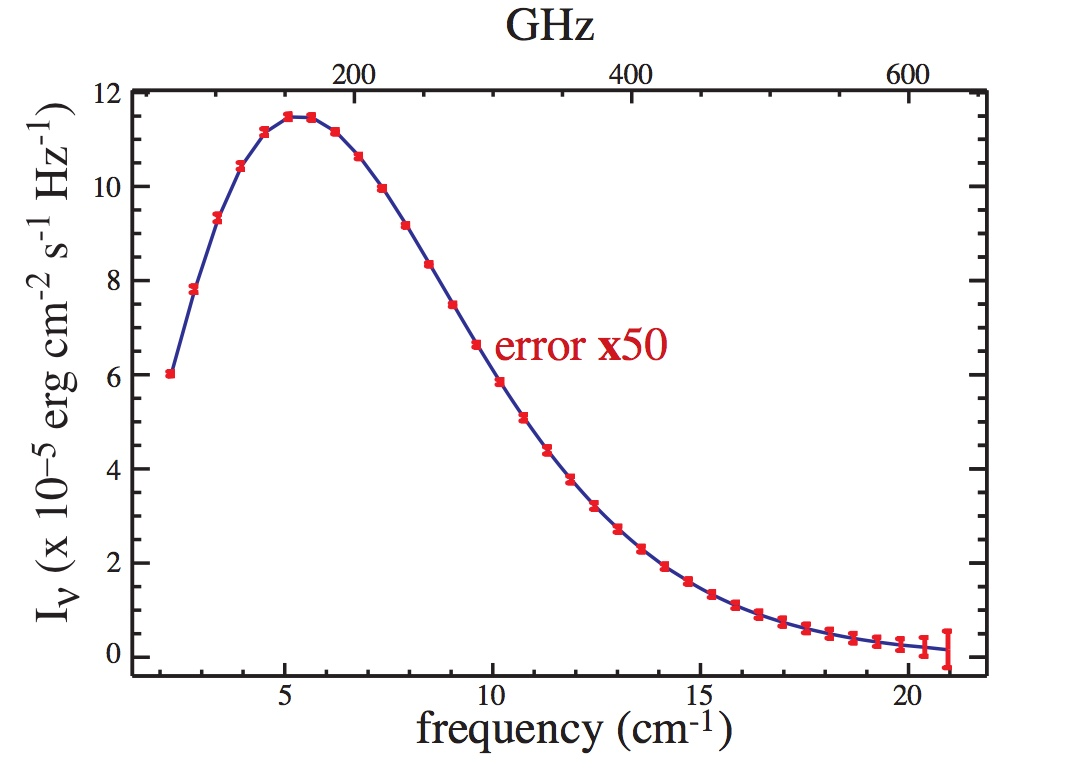
\includegraphics[height=8cm]{blackbody}}
\caption{}
\label{cobe_blackbody}
\end{figure}


\begin{figure}
\centering
    \textbf{The Cosmic Microwave Background anisotropies measured by COBE, WMAP and Planck}\par\medskip
\centering
   {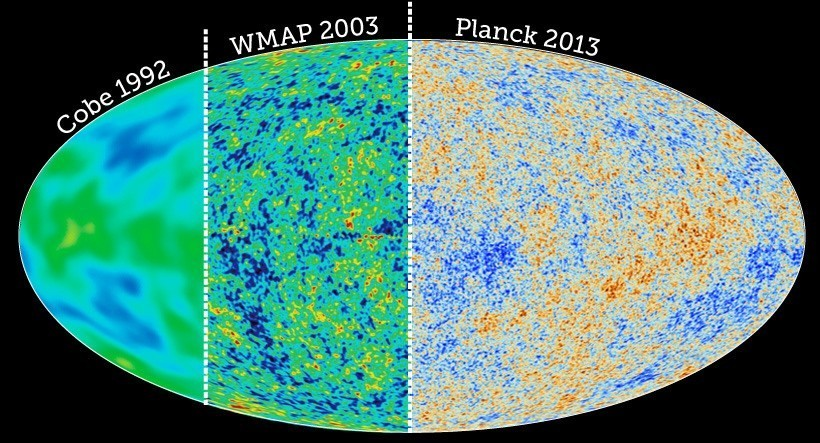
\includegraphics[width=.75\textwidth]{cmb1.jpg}}


\caption{The COBE, WMAP and Planck missions measured the CMB anisotropies with increasing accuracy. COBE, the first CMB satellite, measured fluctuations to scales of 7$^\circ$. WMAP was able to measure resolutions down to 0.3$^\circ$ in five different frequency bands, with Planck measuring all the way down to just 5 arcminutes (0.07$^\circ$) in nine different frequency bands in total.  (NASA/COBE/DMR; NASA/WMAP SCIENCE TEAM; ESA AND THE PLANCK COLLABORATION)}
\label{cobe_wmap_planck}
\end{figure}


\begin{figure}
\centering
    \textbf{Orbits of different  configurations of BBH}\par\medskip
\centering
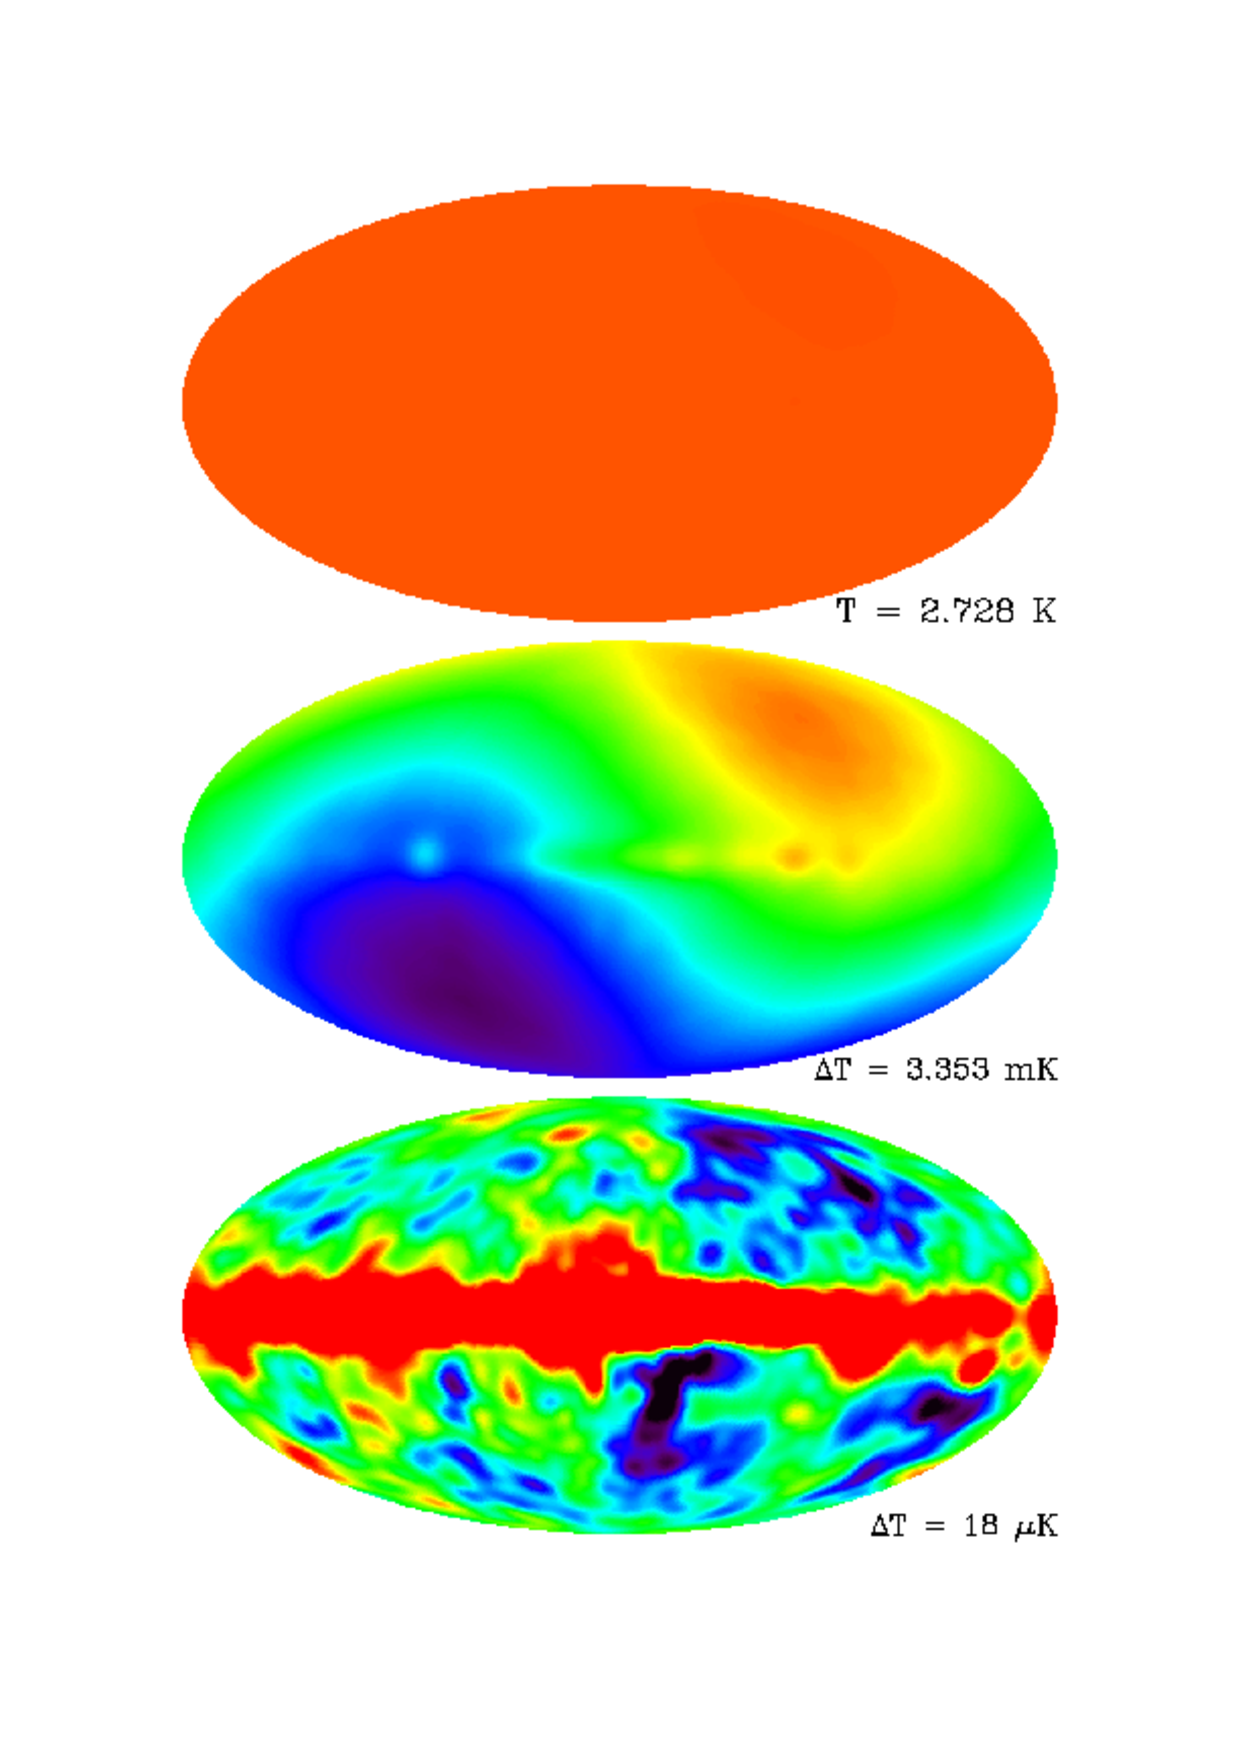
\includegraphics[scale =0.3]{mono_di_cobe}
\caption{The microwave sky as seen by the COBE DMR (differential microwave radiometer) instrument. The top panel shows the microwave sky as seen on a linear tem- perature scale including zero. No anisotropies are visible in this image, because the CMB monopole at 2.725K dominates. In the middle panel, the monopole component has been subtracted. Apart from some slight contamination from the galaxy near the equator (corre- sponding to the plane of our Galaxy), one sees only a nearly perfect dipole pattern, owing to our peculiar motion with respect to the rest frame defined by the CMB. In the bottom panel, both the monopole and dipole components have been removed. Except for the galactic contamination around the equator, one sees the cosmic microwave background anisotropy along with some noise. (Credit: NASA/COBE Science Team)}
\label{cobe_map}
\end{figure}

\newpage


\section{Content of the Universe} 
It is often said that our Universe is made up of $68.8$\% of Dark Energy, and $26.8 $\% by Dark Matter and $4.9 $\% of ordinary matter, but what do we really mean by that?\\
In this section we explain where the components of our Universe (Dark Matter, baryonic matter, Dark Energy, curvature)  arise from and how they are related with each others. 
The assumptions and the theoretical framework that we are going to explain will be then used to analyze the observations of the CMB.\\
We assume that the observable properties of the Universe are isotropic and there is not a preferred direction. 
Therefore, the Universe is assumed to be homogenous and isotropic at enough large scales $> 100$ Mpc, at least up to the observable universe.\\
Another important assumption is that there exists a class of observers at rest with respect to the Cosmic Microwave Background \citep{bartelmannStandardModelCosmology}.
Let us clarify this concept. 
After subtracting the average temperature of the CMB from its spectrum, a moving observer with respect with the CMB will see a dipole pattern, where the blue-shifted photons come from the direction the observer is moving toward to and the red-shifted photons from the opposite direction.
Since Earth is not at rest with respect to the CMB, the satellite COBE measured the dipole pattern showed in the second panel in Figure (\ref{cobe_map}).\\
Given these assumptions, the most general metric $g_{\mu \nu}$ satisfying homogeneity and isotropy is the Friedmann–Lemaître–Robertson–Walker (FLRW) metric written here in terms of the invariant geodesic distance $\dd s ^2 = g_{\mu \nu} \dd x^{\mu} \dd x^{\nu}$:
\begin{equation}
\label{metric}
\dd s ^2 = -c ^2 \dd t^2 + a^2 (t) \qty( \frac{1}{1-k \, r^2} \dd r^2 + r^2 \dd \Omega ^2 )  
\end{equation}
where $k$ is the spatial curvature and $a(t)$ is the scale factor.
Notice that the FLRW metric has $g_{0 i}=0$ due to the isotropy.
\\ % comments on the redshift, metric, what spatially flat means
If we assume the correctnes of the General Theory of Relativity, we can use the Einstein's field equations
\begin{equation}
\label{einstein_eq}
R_{\mu \nu} - \dfrac{1}{2} R \, g _{\mu \nu} + \Lambda g_{\mu \nu}= \dfrac{8 \pi G}{c^4} \, T_{\mu \nu}
\end{equation}
in order to evolve the FLRW metric.
The Einstein's field equations relate how the geometry of spacetime (left hand side) changes with the presence of masses and energy (right hand side).
The most general fluid consistent with the assumption of homogeneity and isotropy is a perfect fluid, one in which an observer comoving with the fluid would see the universe around it as isotropic \citep{garcia-bellidoAstrophysicsCosmology2000}. Therefore, the energy-momentum tensor $T_{\mu \nu}$ can be written as
\begin{equation}
\label{energy-momentum-tensor}
T^{\mu \nu } = (p + \rho c^2)u ^{\mu} u^{\nu}+p g^{\mu \nu} 
\end{equation}
where $\rho$ and $p$ are, respectively, the mass density and the pressure of the fluid.\\
Solving (\ref{einstein_eq}) for $\mu= 0=\nu$ using the above definition (\ref{energy-momentum-tensor}), gives us the Friedmann equation:
\begin{equation}
\label{firedmann_eq}
\begin{split}
H^2 = \qty(\frac{\dot{a}}{a})^2 = \dfrac{8 \pi G}{3} \rho -\dfrac{k \, c^2}{a^2} + \frac{\Lambda \, c^2}{3}
\end{split}
\end{equation}
where $\dot{a}$ is the time derivative of the scale factor.\\
And the conservation of energy momentum tensor $\nabla_\mu T^{\mu 0} =0 $ becomes:
\beq
\label{energy_cons}
\dv[]{}{t}\qty(\rho c^2 a^3) + p \dv[]{}{t} \qty(a^3)  = 0
\eeq
Solving for radiation $\rho c^2 = p/3$
\[
\dot{\rho}  + 4 \frac{ \dot{a}}{a} \rho =0
\]
 And solving for matter $\rho c^2 << p$
 \[
 \dot{\rho}  + 3 \frac{ \dot{a}}{a} \rho =0
 \]
Solving this for matter $\rho_m << p_m$ (or \emph{dust}) and for radiation $\rho_r = p_r/3$ gives
\begin{equation}
\begin{split}
\rho_m = \rho_{m 0} a^{-3} \hspace{1.5cm} \rho_r = \rho_{r 0} a^{-4} \notag
\end{split}
\end{equation}
where $\rho_{m 0}$ and $\rho_{r 0}$ are the matter density and radiation density evaluated today $t = t_0$, $a(t_0) = a_0 =1$.\\
We now rewrite equation (\ref{firedmann_eq}) as
\begin{equation}
H ^2 = H_0 ^2 \qty[
\dfrac{8 \pi G}{3 H_0 ^2} \rho_{m 0} a^{-3}+
\dfrac{8 \pi G}{3 H_0 ^2} \rho_{r 0} a^{-4}+ 
\dfrac{-k \, c^2}{H_0 ^2} a^{-2} + \dfrac{\Lambda \, c^2}{3 H_0 ^2}
] \notag
\end{equation}
where we defined $H_0 = H(t_0)$.\\
\beq
\Omega_\Lambda = \dfrac{\Lambda c^2}{3} \qquad \Omega_k = -  \dfrac{k c^2}{H_0 ^2} \qquad
\Omega_m = \dfrac{8 \pi G}{3 H_0 ^2} \rho_{m 0} \qquad \Omega_r =\dfrac{8 \pi G}{3 H_0 ^2} \rho_{r 0}
\eeq
evaluating the Friedmann equation (\ref{firedmann_eq}) today we obtain the cosmic sum rule
\begin{equation}
\label{cosmic_rule}
\Omega_{\Lambda} + \Omega_{m} + \Omega_k + \Omega_{r} = 1
\end{equation}







\section{Phenomenology of the Fluctuations}
The Cosmic Microwave Background is the image of the fluctuations of a dense and hot fluid made of matter and radiation.
Before the release of the CMB at $z > 1100$ the electromagnetic radiation is firmly coupled (both energetically and kinetically) to the baryons and it is possible to describe the behavior of such a system by using solving the equations of relativistic hydrodynamics and the Einstein's field equations (\ref{einstein_eq}) with small density $\delta \rho$, pressure $\delta p$ and gravitational potential perturbations $\delta \Phi$.
The full general-relativistic description of the photon-matter fluid requires a complicated treatment[BAUMANN].
However, it is possible to qualitatively discuss the phenomena occurring in the CMB fluid and the effects on the temperature fluctuations $\Theta = \delta T / T_0$.
\subsection{Sachs-Wolfe effect}
As a consequence of the Einstein's equivalence principle, photons that escape from a gravitational field are redshifted.
If we consider the fluctuations of the CMB on large scales, the photons that tries to escape from the gravitational well created by matter are redshifted.

\subsection{Acoustic oscillations}
At the time of recombination
Dark Matter is randomly distributed
if a portion of photon-baryon fluid is in a potential well of the dark matter, it will fall to the center of the well
gravity compresses the photon-baryon fluid
pressure starts to rise
the pressure is sufficient to cause the fluid to expand outward
the pressure drops until gravity causes the photon-baryon fluid to fall inward again\\
Gravity tries to compress the fluid in potential wells.
Photon pressure resists compression resulting in acoustic oscillations
System is equivalent to a mass on a spring falling under gravity
What is doing the pushing that compresses the fluid? Gravity.

The photon-baryon fluid is sitting in the gravitational potential wells that are the seeds of structure in the universe.  As gravity tries to compress the fluid, radiation pressure resists resulting in acoustic oscillations.  Because it acts to resist compression, we will represent the radiation pressure abstractly as springs.  Likewise we will represent the inertia of the fluid, or loosely speaking its mass (really energy density), as massive balls falling under gravity:\\

Modes caught at extrema of their oscillations become the peaks in the CMB power spectrum.  They form a harmonic series based on the distance sound can travel by recombination, called the sound horizon.  The first peak represents the mode that compressed once inside potential wells before recombination, the second the mode that compressed and then rarefied, the third the mode that compressed then rarefied then compressed, etc



\subsection{Damping}
The temperature fluctuations are damped due to collisions between the baryons and the photons that dissipate energy, and the expansion of the universe.\\
The damping scale provides another standard ruler for the curvature test
The physical scale of the damping depends on the baryon density through the mean free path
And the matter density through the time available for the photons to random walk.
If we can calibrate the distance CMB photons random walk during recombination, we have another standard ruler for the angular diameter distance test of the spatial curvature of the universe.  Remember that we measure its angular scale in the power spectrum itself.

Alternatively, if we know the curvature of the universe we can infer the physical distance the photons travel.  In the standard model, the physical distance depends only on the baryon density and the dark matter density (matter-radiation ratio).  Since all three (curvature, baryons density and matter radiation) are measured by the positions and heights of the peaks themselves, the damping tail provides a beautiful consistency test for the standard model.

Let's see how that works.

Microphysically, the distance photons can travel is related to a random walk process.  Remember that the photons have a certain mean free path in the baryons defined as the average distance the photon travels before Thomson scattering off a free electron:\\
Raising the number of baryons, decreases the mean free path and hence shortens the distance photons can travel at recombination.  Finally the full distance also depends on the amount of time the photons have to random walk and hence the age of the universe at recombination.  Remember that the age is determined by the dark matter density.  Mathematically, the length is roughly the geometric mean of the mean free path and the distance light can travel without obstruction (the horizon scale).
\begin{comment}
    This text will not be displayed.

 by starting from the continuity and Euler equation for a photon fluid with  number density $n$, energy density $u$ and pressure $p$:
\begin{equation}
\label{hydro}
\dot{n} + n_0 \vec{\nabla} \cdot \vec{v} = 0 \qquad
\dot{\vec{v}} = - c^2 \dfrac{\vec{\nabla} \delta p}{p_0 + u_0} - \vec{\nabla} \delta \Phi
\end{equation}
where $v$ is the streaming velocity of the perturbations and the subscript $_0$ indicates the background average values of th correspondent quantities.\\
For a photon gas we know that
\begin{equation}
n \propto T ^3 \qquad u \propto T^4 \qquad p  = \dfrac{u}{3}
\end{equation}
So, the temperature fluctuations are related to the number density, energy density and pressure as follow:
\begin{equation}
\dfrac{\delta n}{n_0} = 3 \Theta \qquad
\dfrac{\delta u}{u_0} = 4 \Theta = \dfrac{\delta p}{p_0}
\end{equation}
We can rewrite eq.(\ref{hydro}) in terms of the temperature fluctuations:
\begin{equation}
\dot{\Theta} + \nabla \cdot \vec{v} = 0 \qquad \dot{\vec{v}} = - c^2 \vec{\nabla} \Theta - \vec{\nabla} \delta \Phi
\end{equation}
where we used $p_0 + u_0 = 4 p_0$

\begin{itemize}
\item hydrodynamics \citep{huLectureNotesCMB2008}
page 14 eq 49 to page 17 eq 71\\
skip doppler effect
\item gravito acoustic oscillations page 19 up to eq 82 , justify briefly constant potential in page 20
% if stress perturbations are negligible compared with density perturbations ( δp ≪ δρ ) then the potential will remain constant in periods where the background equation of state p/ρ is constant
\item page 20 and 21 up to eq92 important comment 
%The consequence is that overdense regions where Ψ is negative (potential wells) are cold spots in the effective temperature.
\item baryonic effect
\end{itemize}
\end{comment}


\section{Comments on the results and plots of the CMB spectrum}
We have seen in section 3 how general relativity and the density parameters  characterize the content of our Universe,  in section 4 the dynamics of the CMB photons is affected by matter.
We want to link the previous theoretical results to the observations of the temperature fluctuations of the CMB sky.\\
The spherical harmonics $Y^{m} _{l} (\theta, \phi)$ compose a set of orthonormal functions on the sky.\\
So if $T(\theta,\phi)$ is the temperature at position $(\theta,\phi)$, it is possible to decompose the temperature into a series:
\begin{equation}
T(\theta, \phi) = \sum _{l, m} a_{lm} Y^{m} _l (\theta, \phi)
\end{equation}
Due to the orthonormality of the spherical harmonics
\begin{equation}
a_{lm} = \int _0 ^{2 \pi} \dd \phi \int _0  ^{\pi} \dd \theta \,
\sin \theta \, T(\theta, \phi) \, Y^{m} _l (\theta, \phi)
 \end{equation}
 We define the power spectrum of the temperature map as 
 \begin{equation}
 C_l = \dfrac{1}{2l+1} \sum _{m=-l} ^{l} |a_{lm}|^2
 \end{equation}
The measured temperature power spectrum is shown in Figure(\ref{temp_pow_spect})
%
%
%
\begin{figure}
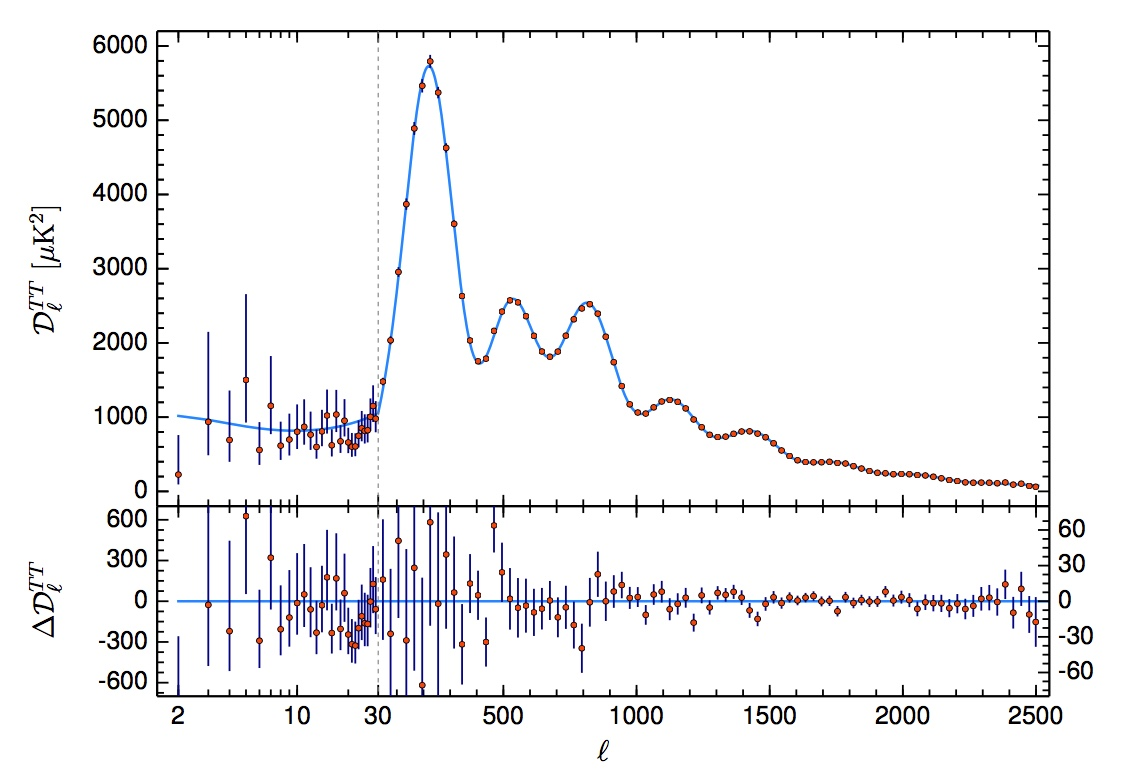
\includegraphics[width=0.9\textwidth]{planck2018}
\caption{Planck 2018 temperature power spectrum. $\mathcal{D}^{TT}_l = l(l+1)C_l$ (arXiv:1807.06209v1)}
\label{temp_pow_spect}
\end{figure}
%
%
%
The Sachs-Wolfe effect is dominant on large scales, i.e. small l.\\
The first peak is at $l \approx 200$ and the  acoustic oscillations take place.
The damping effect is evident for $l>10^{3}$.\\

\subsection{Dark Energy and Curvature}

Position of peaks mainly sensitive to curvature
Shapes fixed by the physical density of matter and baryons
Missing or "dark energy" plays a small roll in the position of peaks
As advertised, the position of that first peak in the power spectrum of the anisotropies, and indeed all of the peaks, depend sensitively on the spatial curvature of the universe.   As the curvature of the universe decreases (and in fact becomes negative in the yellow curve below)\\
the peaks move to smaller angles (higher multipole l) while preserving their shape.  Cosmologists fraction of the critical density in matter Omegam so that as 1-Omegamincreases from zero, the universe becomes increasingly negatively curved if there is no other forms of "missing energy" that we've missed in our accounting.

Caveats:

In the blue curve, we assume that there is indeed a form of "missing" or dark energy in a cosmological constant that makes the universe flat despite a sub-critical density of matter.  We see that the positions mainly care about the curvature of the universe but there is a small shift to larger angular scales (lower multipoles) through the introduction of a cosmological constant.  This is because the cosmological constant produces a small change in the distance light can travel since recombination, a fact that is related to its well known effect on the age of the universe. 

Note that in the above figure we assume that the physical density of the matter (Omegamh2) is fixed.  This is different from saying its fraction of the critical density (Omegam) is fixed since the Hubble constant (h), or expansion rate today, enters into the definition of the critical density.  Given our current uncertainties about the physical density of the matter, the distance that sound can travel by recombination is currently uncertain, a fact related to the matter's effect on the age of the universe at recombination.  Likewise we have assumed that the physical density of the baryons  (Omegabh2) is fixed.  Baryons lower the speed of sound in the medium and hence also affect the distance sound can travel.  Luckily both of these quantities dramatically change the shape of the peaks as we shall see.  They will be measured once the higher peaks are detected and will no longer confuse the measurement of the curvature.   As it turns out, the sound horizon is not a standard ruler but rather a standardizeable ruler.
\begin{figure}
\begin{center}
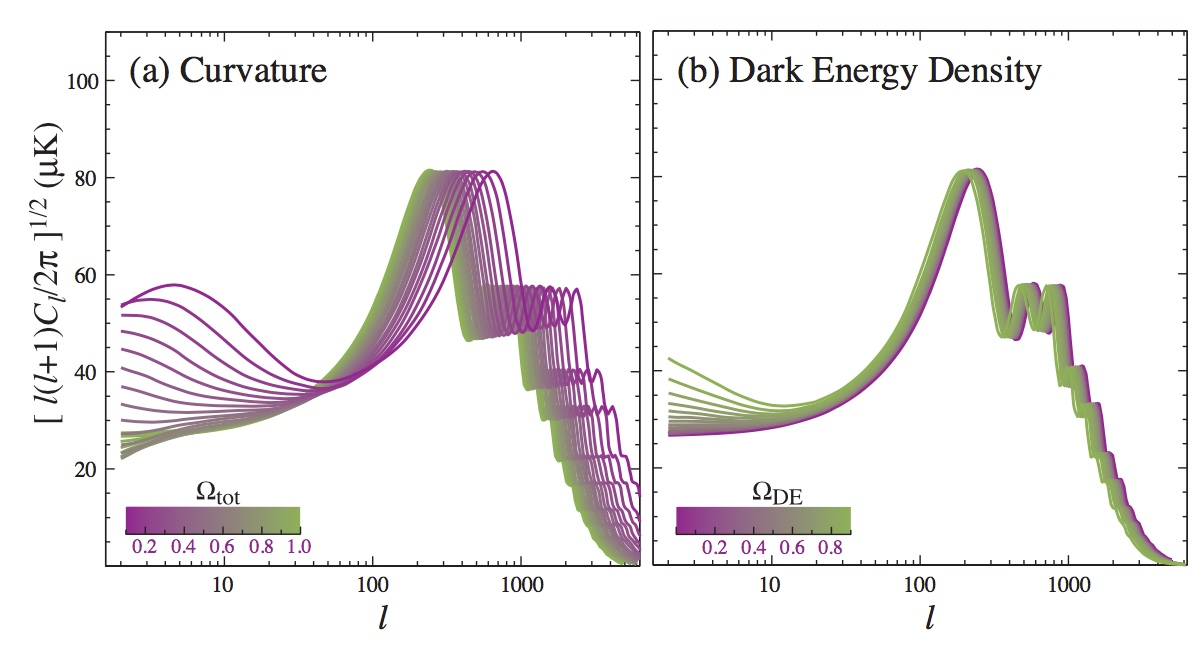
\includegraphics[width=\textwidth]{curvature_de}
\caption{}

\end{center}
\label{DE_curv}
\end{figure}

\subsection{Dark Matter and Baryons}
Baryons (or ordinary matter) load down the photon-baryon plasma and add inertial (and gravitational) mass to the oscillating system.

Their effect on the acoustic peaks is easy to understand.  Remember what happens when you add mass to a spring and let it fall in the gravitational field of the Earth.  With more mass loading the spring, it falls further before pulled back by the spring.  On the other hand, it rebounds to the same position it started from. 

Since the odd numbered (first, third, fifth...) acoustic peaks are associated with how far the plasma "falls" into gravitational potential wells (how much the plasma compresses), they are enhanced by an increase in the amount of baryons in the universe.   The even numbered peaks (second, fourth, sixth) are associated with how far the plasma "rebounds" (how much the plasma rarefies).  Thus with the addition of baryons the odd peaks are enhanced over the even peaks.  For example, baryons make the first acoustic peak much larger than the second.  The more baryons the more the second peak is relatively suppressed. 
\par

%http://background.uchicago.edu/~whu/intermediate/baryons2.html
\paragraph{image}
Power spectrum shows baryons enhance every other peak.
Second peak is suppressed compared with the first and third
Additional effects on the peak position and damping yield consistency checks
When we do the full calculation of the power spectrum, the basic physics of a mass on the spring appears as advertised.   The odd numbered acoustic peaks in the power spectrum are enhanced in amplitude over the even numbered ones as we increase the baryon density of the universe.\\
Note: Cosmologists label the baryon density in terms of its fraction of the critical density Wbtimes the Hubble constant squared (in units of 100 km/s/Mpc) to get something proportional to the physical density of the baryons.]

There are two other related effects due to the baryons:  since adding mass to a spring slows the oscillation down, adding baryons to the plasma decrease the frequency of the oscillations pushing the position of the peaks to slightly higher multipoles l.

Baryons also affect the way the sound waves damp and hence how the power spectrum falls off at high multipole moment lor small angular scales as we will see later.

The many ways that baryons show up in the power spectrum imply that the power spectrum has many independent checks on the baryon density of the universe.  The baryon density is a quantity that the CMB can measure to exquisite precision.

\paragraph{dark matter}
Second peak is observed to be substantially lower than first peak
Dark baryons of at least the big-bang nucleosynethesis density required
Although we cannot yet claim that the second peak is as precisely measured as the first, we can say that (assuming it exists!) it is definitely of lower amplitude than the first:\\
The current data indicate that the baryon density is around Omegabh2=0.02 This value is interesting since it is also the baryon density inferred from the abundance of deuterium at high redshift in quasar absorption lines and the theory of big-bang nucleosynthesis.  We now have an additional and independent line of evidence that there are missing baryons in the universe - i.e. that most the baryons are not in stars.   Once the second and higher peaks are definitively measured, CMB constraints on the baryon density will sharpen considerably (ultimately to a few percent accuracy).  Needless to say it will be interesting to see how these comparisons shape up as the data improve.
\paragraph{dark}
Raising the dark matter density reduces the overall amplitude of the peaks.
Lowering the dark matter density eliminates the baryon loading effect so that a high third peak is an indication of dark matter.
With three peaks, its effects are distinct from the baryons
Measuring the dark matter density resolves the main ambiguity in the curvature measurement
As advertised the acoustic peaks in the power spectrum are sensitive to the dark matter density in the universe.  (Formally, the matter to radiation ratio but the radiation density is fixed in the standard model.)\\
As we raise the physical density of the dark matter, Wmh2, the driving effect goes away at a given peak such that its amplitude decreases.  Although this effect changes the heights of all the peaks, it is only separable from the baryonic effects with at least three peaks.  Note that decreasing the matter density also affects the baryon loading since the dark matter potential wells go away leaving nothing for the baryons to fall into. Having a third peak that is boosted to a height comparable to or exceeding the second peak is an indication that dark matter dominated the matter density in the plasma before recombination. Note that the self-gravity of the photons and baryons still plays a role in the first and second peaks so that the third peak is the cleanest test of this behavior.

Notice also that the location of the peaks, and that of the first peak in particular, changes as we change the dark matter density.  The matter to radiation ratio also controls the age of the universe at recombination and hence how far sound can travel relative to how far light travels after recombination.  This is the leading order ambiguity in the measurement of the spatial curvature of the universe.  We see here that that ambiguity will be resolved when at least three peaks are precisely measured.





\begin{figure}
\begin{center}
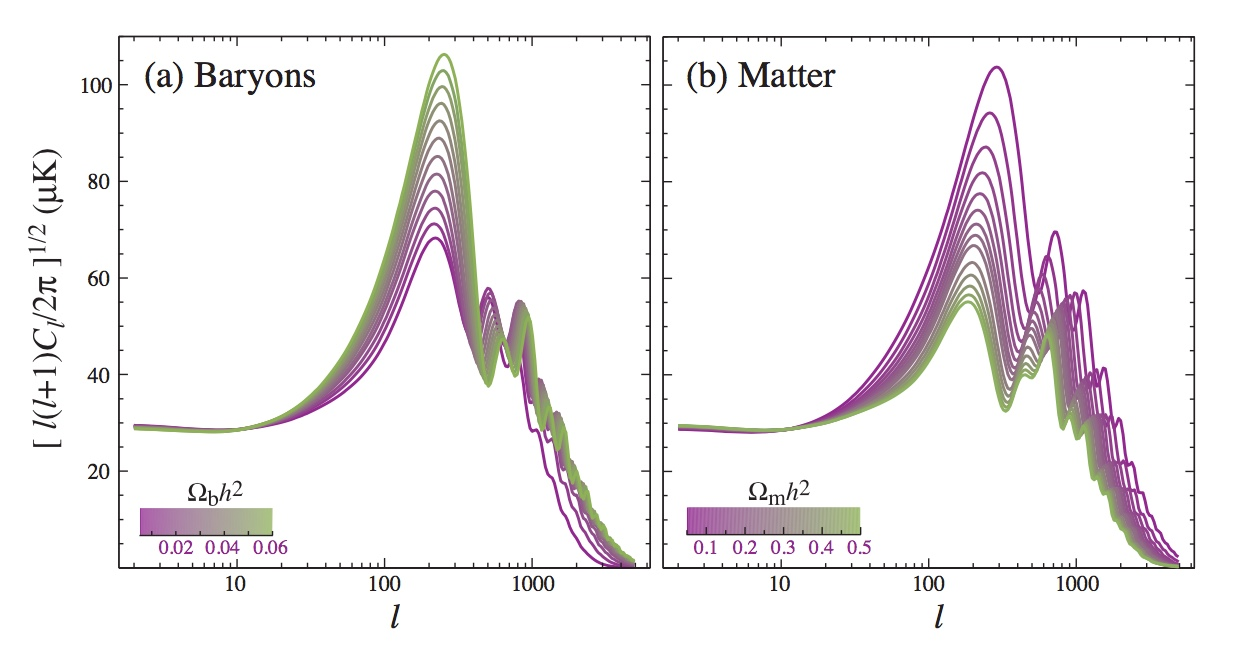
\includegraphics[width=\textwidth]{baryon_m}
\caption{aa}
\end{center}
\label{DM_bar}
\end{figure}
\section{Conclusion}
nn
\citep{padmanabhanDetectingDarkMatter2005}



\bibliographystyle{plain}
\bibliography{dark_1}
\end{document}
